% Clase del documento
\documentclass[12pt,twoside,titlepage]{report}





%%%%%%%%%%%%%%%%%%%%%%% Paquetes %%%%%%%%%%%%%%%%%%%%%%%

\usepackage[a4paper,bindingoffset=3mm,bottom=35mm]{geometry}


% Usad \usepackage[dvips]{graphicx} o \usepackage[pdftex]{graphicx} (no ambos)
%\usepackage[dvips]{graphicx} %%% para LaTeX. Las figuras deben estar en formato eps

\usepackage[colorlinks=true,pdftex]{hyperref}   %%% Opcional. Para incluir marcadores y enlaces en el pdf
\usepackage[pdftex]{graphicx}  %%% para pdflatex. Las figuras pueden estar en pdf, jpg, svg y otros formatos


\usepackage[spanish]{babel}

%\usepackage[latin1]{inputenc} % Usad en WinEdt/MikTex
\usepackage[utf8]{inputenc} % Usad en overleaf

%\usepackage[T1]{fontenc}


% Algunos paquetes útiles

\usepackage{amsmath,amssymb}
\usepackage{hyperref}
\usepackage{xcolor}
\usepackage{afterpage}
\usepackage{paralist}
\usepackage{array}
\usepackage{enumerate}
\usepackage{paralist}
\usepackage{enumitem}
\usepackage{float}
\usepackage{setspace}
\usepackage{listings}
\usepackage{algorithm}
\usepackage{algorithmic}
\usepackage{fancyhdr}
\usepackage{rotating}
\usepackage{multirow}


% Otros paquetes

\usepackage{quotchap}
\usepackage{lipsum}

%%%%%%%%%%%%%%%%%%%%%%%%%%%%%%%%%%%%%%%%%%%%%%%%%%%%%%%%






%%%%%%%%%%%%%%%%%%%%%%% Definiciones básicas %%%%%%%%%%%%%%%%%%%%%%%

\newcommand{\nombreautor}{Jorge Moreno Fernández}
\newcommand{\nombretutor}{Michel Maes Bermejo}
\newcommand{\nombrecotutor}{Micael Gallego Carrillo}
\newcommand{\titulotrabajo}{CoWordle, un juego competitivo online}
\newcommand{\escuela}{Escuela Técnica Superior\\de Ingeniería Informática}
\newcommand{\escuelalargo}{Escuela Técnica Superior de Ingeniería Informática}
\newcommand{\universidad}{Universidad Rey Juan Carlos}
\newcommand{\fecha}{Fecha}
\newcommand{\grado}{Grado en Ingeniería Informática}
\newcommand{\curso}{Curso 2022-2023}
\newcommand{\logoUniversidad}{logoURJC.pdf} % logoURJC.eps

%%%%%%%%%%%%%%%%%%%%%%%%%%%%%%%%%%%%%%%%%%%%%%%%%%%%%%%%%%%%%%%%%%%%






%%%%%%%%%%%%%%%%%%%%%%%%% Otras definiciones %%%%%%%%%%%%%%%%%%%%%%%%%%

% Definiciones de colores (para hidelinks)
\definecolor{BlueLink}{rgb}{0.165,0.322,0.745}
\definecolor{PinkLink}{rgb}{0.8,0.22,0.5}
\definecolor{gray}{rgb}{0.6,0.6,0.6}


% Enlaces
\hypersetup{hidelinks,pageanchor=true,colorlinks,citecolor=PinkLink,urlcolor=black,linkcolor=BlueLink}


\newcommand\blankpage{%
    \newpage
    \null
    \thispagestyle{empty}%
    %\addtocounter{page}{-1}%
    \newpage}


% Texto referencias
\addto{\captionsspanish}{\renewcommand{\bibname}{Bibliografía}}

% Texto Índice de tablas
\addto\captionsspanish{
\def\tablename{Tabla}
\def\listtablename{\'{I}ndice de tablas}
}


\floatname{algorithm}{Algoritmo}

\newfloat{algorithm}{t}{lop}

%% Etiquetas de comentarios (tutor/alumno)
\newif\ifdraft
\drafttrue
\usepackage{subcaption}
\newcommand{\nb}[2]{
	{
		{\color{black}{
				\small\fbox{\bfseries\sffamily\scriptsize#1}
				{\sffamily\small$\triangleright~${\it\sffamily\small #2}$~\triangleleft$}
	}}}
}

\ifdraft
\newcommand\tutor[1]{\nb{Tutor}{\color{red}#1}}
\newcommand\alumno[1]{\nb{Alumno}{\color{blue}#1}}
\newcommand\cotutor[1]{\nb{Co-tutor}{\color{green}#1}}
\newcommand{\fixme}[1]{{\textcolor{red}{[FIXME] #1}}\xspace}
\newcommand{\cn}{{\color{violet}[citation required]}}

\else
%\usepackage[disable]{todonotes}
\newcommand\tutor[1]{}
\newcommand\alumno[1]{}
\newcommand\cotutor[1]{}
\newcommand{\fixme}[1]{}
\newcommand{\cn}{}

\fi






%\newenvironment{pseudocodigo}[1][htb]
%  {\renewcommand{\algorithmcfname}{Pseudocódig}% Update algorithm name
%   \begin{algorithm}[#1]%
%  }{\end{algorithm}}
  
%%%%%%%%%%%%%%%%%%%%%%%%%%%%%%%%%%%%%%%%%%%%%%%%%%%%%%%%%%%%%%%%%%%%





%%%%%%%%%%%%%%%%%%%%%%% Estilo de código (en Python) %%%%%%%%%%%%%%%%%%%%%%%

\definecolor{bg}{rgb}{0.95,0.95,0.95}
\definecolor{mydeepteal}{rgb}{0.16,0.22,0.23}
\definecolor{myteal}{rgb}{0.31,0.44,0.46}
\definecolor{mymediumteal}{rgb}{0.41,0.58,0.60}

\DeclareFixedFont{\ttb}{T1}{txtt}{bx}{n}{12} % for bold
\DeclareFixedFont{\ttm}{T1}{txtt}{m}{n}{12}  % for normal


%\newcommand*{\FormatDigit}[1]{\textcolor{mydeepteal}{#1}}
\newcommand*{\FormatDigit}[1]{\textcolor{black}{#1}}

% Python style for highlighting
\newcommand\mypythonstyle{\lstset{
language=Python,
basicstyle=\ttfamily\small,
%basicstyle=\linespread{1.0}\footnotesize\ttm,
otherkeywords={self},             % Add keywords here
keywordstyle=\bfseries\ttfamily\color{myteal},
%keywordstyle=\ttb\color{myteal},
commentstyle=\itshape\color{myteal},
stringstyle=\color{mydeepteal},
emph={MyClass,__init__},          % Custom highlighting
emphstyle=\ttb\color{mydeepteal},    % Custom highlighting style
% Any extra options here
showstringspaces=false,            %
backgroundcolor=\color{bg},
rulecolor = \color{bg},
%identifierstyle=\color{deepgreen},
breaklines=true,
numbers=left,
numbersep=5pt,
numberstyle=\tiny,
tabsize=4,
xleftmargin=1em,
frame = single,
framesep = 3pt,
framextopmargin=0pt,
framexbottommargin=0pt,
framexleftmargin=0pt,
framexrightmargin=0pt,
fontadjust=true,
basewidth=0.55em, % compactness of code
upquote=true,
}}

% Python environment
\lstnewenvironment{mypython}[1][]
{
\mypythonstyle
\lstset{#1}
}
{}

\newcommand\mypythonstylenormalinline{\lstset{
language=Python,
basicstyle=\ttfamily\normalsize,
%basicstyle=\linespread{1.0}\footnotesize\ttm,
otherkeywords={self},            % Add keywords here
keywordstyle=\bfseries\ttfamily\color{myteal},
%keywordstyle=\ttb\color{myteal},
commentstyle=\itshape\color{mymediumteal},
stringstyle=\color{mydeepteal},
emph={MyClass,__init__},          % Custom highlighting
emphstyle=\ttb\color{mydeepteal},    % Custom highlighting style
% Any extra options here
showstringspaces=false,            %
backgroundcolor=\color{bg},
rulecolor = \color{bg},
%identifierstyle=\color{deepgreen},
breaklines=false,
numbers=left,
numbersep=5pt,
numberstyle=\tiny,
tabsize=4,
xleftmargin=0em,
frame = single,
framesep = 3pt,
framextopmargin=0pt,
framexbottommargin=0pt,
framexleftmargin=0pt,
framexrightmargin=0pt,
fontadjust=true,
%basewidth=0.55em, % compactness of code
upquote=true,
}}

\newcommand\mypythoninline[1]{{\mypythonstylenormalinline\lstinline!#1!}}

%%%%%%%%%%%%%%%%%%%%%%%%%%%%%%%%%%%%%%%%%%%%%%%%%%%%%%%%%%%%%%%%%%%%%%%%%%%%%%


%%%%%%%%%%%%%%%%%%%%%%% Estilo de código (en Typescript) %%%%%%%%%%%%%%%%%%%%%%%

% Javascript style for highlighting
\lstdefinelanguage{Typescript}{
  keywords={break, case, catch, continue, debugger, default, delete, do, else, false, finally, for, function, if, in, instanceof, new, null, return, switch, this, throw, true, try, typeof, var, void, while, with, const, as, extends},
  morecomment=[l]{//},
  morecomment=[s]{/*}{*/},
  morestring=[b]',
  morestring=[b]",
  ndkeywords={class, export, boolean, throw, implements, import, this},
  keywordstyle=\color{blue}\bfseries,
  ndkeywordstyle=\color{darkgray}\bfseries,
  identifierstyle=\color{black},
  commentstyle=\color{purple}\ttfamily,
  stringstyle=\color{red}\ttfamily,
  sensitive=true
}

% \lstset{
%    language=JavaScript,
%    backgroundcolor=\color{lightgray},
%    extendedchars=true,
%    basicstyle=\footnotesize\ttfamily,
%    showstringspaces=false,
%    showspaces=false,
%    numbers=left,
%    numberstyle=\footnotesize,
%    numbersep=9pt,
%    tabsize=2,
%    breaklines=true,
%    showtabs=false,
%    captionpos=b
% }

% Typescript style for highlighting
\newcommand\mytypescriptstyle{\lstset{
language=Typescript,
basicstyle=\ttfamily\small,
%basicstyle=\linespread{1.0}\footnotesize\ttm,
otherkeywords={self},             % Add keywords here
keywordstyle=\bfseries\ttfamily\color{myteal},
%keywordstyle=\ttb\color{myteal},
commentstyle=\itshape\color{myteal},
stringstyle=\color{mydeepteal},
emph={MyClass,__init__},          % Custom highlighting
emphstyle=\ttb\color{mydeepteal},    % Custom highlighting style
% Any extra options here
showstringspaces=false,            %
backgroundcolor=\color{bg},
rulecolor = \color{bg},
%identifierstyle=\color{deepgreen},
breaklines=true,
numbers=left,
numbersep=5pt,
numberstyle=\tiny,
tabsize=4,
xleftmargin=1em,
frame = single,
framesep = 3pt,
framextopmargin=0pt,
framexbottommargin=0pt,
framexleftmargin=0pt,
framexrightmargin=0pt,
fontadjust=true,
basewidth=0.55em, % compactness of code
upquote=true,
}}

% Typescript environment
\lstnewenvironment{mytypescript}[1][]
{
\mytypescriptstyle
\lstset{#1}
}
{}

%%%%%%%%%%%%%%%%%%%%%%%%%%%%%%%%%%%%%%%%%%%%%%%%%%%%%%%%%%%%%%%%%%%%%%%%%%%%%%


%%%%%%%%%%%%%%%%%%%%%%%%%%%% Comandos definidos por el autor 

\newcommand{\transpuesta}{\mbox{\tiny $\mathsf{T}$}}








%%%%%%%%%%%%%%%%%%%%%%%%%%%%%%%%%%%%%%%%%%%%%%%%%%%%%%%%%%%%%%%%%%%%%%%
%                           Inicio del documento                       
%%%%%%%%%%%%%%%%%%%%%%%%%%%%%%%%%%%%%%%%%%%%%%%%%%%%%%%%%%%%%%%%%%%%%%%


\begin{document}

\pagestyle{plain}




%%%%%%%%%%%%%%%%%%%%%%%%%%%%%%%%%%%% Portada %%%%%%%%%%%%%%%%%%%%%%%%%%%%%%%%%%

%\pagenumbering{gobble}
%\pagenumbering{arabic}

% Universidad, Facultad
\begin{titlepage}
	\selectlanguage{spanish}
																																														
																																														
	% logo
	\begin{center}
		\includegraphics[scale=0.7]{\logoUniversidad}
	\end{center}
																																														
	\bigskip
																																														
	\begin{center}
		\begin{LARGE}
			\escuela \\
		\end{LARGE}
	\end{center}
																																														
	\bigskip
	\bigskip
																																														
	% Grado
	\begin{center}
		\begin{large}
			\textbf{\grado}\\
		\end{large}
	\end{center}
																																														
	% Curso
	\begin{center}
		\begin{large}
			\textbf{\curso}\\
		\end{large}
	\end{center}
																																														
	\bigskip
																																														
	\textbf{\begin{center}
		\begin{large}
			\textbf{Trabajo Fin de Grado}
		\end{large}
		\end{center}}
																																														
	\bigskip
	\bigskip
	\bigskip
																																														
	% Nombre del TFG
	\begin{center}
		\textbf{\begin{large}
			\MakeUppercase{\titulotrabajo}\\
			\end{large}}
	\end{center}
																																														
	% Nombre del autor
	\vspace{\fill}
	\begin{center}
		\textbf{Autor: \nombreautor}\\ \smallskip
		% Tutor
		\textbf{Tutor: \nombretutor}\\
		\textbf{Cotutor: \nombrecotutor}\\
		% Añadir segundo tutor si hubiera
																																																																																												
																																																																																												
		\bigskip
																																																																																												
		% Fecha
		%\textbf{\fecha}\\
	\end{center}
\end{titlepage}


%%%%%%%%%%%%%%%%%%%%%%%% Opcional %%%%%%%%%%%%%%%%%%%%%%
%\blankpage

%\thispagestyle{empty}
%\begin{center}

% Nombre del trabajo
%\textbf{\begin{large}
%\MakeUppercase{\titulotrabajo}\\*
%\end{large}}
%\vspace*{0.2cm}
%\vspace{5cm}

% Nombre del autor y del tutor
%\large Autor: \nombreautor \\* \medskip
%\large Tutor: \nombretutor \\*

%\vfill

% Escuela, universidad y fecha
%\escuelalargo \\ \smallskip
%\universidad \\
%\vspace{1cm}
%\fecha \\

%\clearpage

%\end{center}
%%%%%%%%%%%%%%%%%%%%%%%%%%%%%%%%%%%%%%%%%%%%%%%%%%%%%%%%

\hypersetup{pageanchor=true}

\normalsize
\afterpage{\blankpage} % Se deben añadir página en blanco para que lo capítulos de la memoria o estas secciones introductorias empiecen en páginas impares

%%%%%%%%%%%%%%%%%%%%%%%%%%%%%%%%%%%%%%%%%%%%%%%%%%%%%%%%%%%%%%%%%%%%%%%%%%%%%%%





% Estilo de párrafo de los capítulos
\setlength{\parskip}{0.75em}
\renewcommand{\baselinestretch}{1.25}
% Interlineado simple
\spacing{1}

\pagenumbering{Roman}
\setcounter{page}{2}


%%%%%%%%%%%%%%%%%%%%%%%%% Agradecimientos o dedicatoria %%%%%%%%%%%%%%%%%%%%%%%%%%%

\chapter*{Agradecimientos}

Breves agradecimientos o dedicatoria.

\afterpage{\blankpage}

%%%%%%%%%%%%%%%%%%%%%%%%%%%%%%%%%%%%%%%%%%%%%%%%%%%%%%%%%%%%%%%%%%%%%%%%%%%%%%%%%%%






%%%%%%%%%%%%%%%%%%%%%%%%%%%%%%%%%%%% Resumen %%%%%%%%%%%%%%%%%%%%%%%%%%%%%%%%%%%%%%

\chapter*{Resumen}

En esta memoría se va a documentar todo el trabajo realizado para el desarrollo de la aplicación CoWordle, un juego web accesible desde cualquier dispositivo, realizado utilizando las últimas tecnologías web.

CoWordle ha sido la oportunidad perfecta para aprender tecnologías web como WebSockets o Deno, y para realizar un juego multijugador accesible desde cualquier dispositivo que combina el famoso juego Wordle con la competición en tiempo real.

La aplicación cuenta con dos proyectos, por un lado la \textit{webapp}, que permite la visualización de la aplicación utilizando navegadores web. El otro proyecto es el servidor de WebSockets, que realiza la comunicación en tiempo real para todos los jugadores de una partida.

A lo largo de este documento se explican las tecnologías usadas, como SvelteKit o Deno, también se explican aquellos sistemas que se hayan ido creando durante la realización de la aplicación, como los sistemas de tipados para la comunicación Websocket.

\tutor{Repites "También" por segunda vez, inicia, por ejemplo, con "Describiremos los objetivos de este trabajo ..." (que no práctica)} También se describen los objetivos de la práctica y el avance de la aplicación a lo largo del tiempo; la arquitectura escogida, que cuenta con dos proyectos distintos, una webapp y un servidor de WebSockets\tutor{Repites la arquitectura en el resumen};\tutor{No uses ; en un resumen, menos aún continues con una mayúscula} Se explicaran el diseño visual creado inspirado por el Wordle original; Y \tutor{No inicies con un 'Y', usa 'Finalmente, se describirán...'} se describirán cuales son las posibilidades para desplegar la aplicación utilizando GitHub y utilizando Docker.


%\mbox{} \bigskip

\noindent \textbf{Palabras clave}:
\begin{compactitem}
	\item Javascript
	\item Typescript
	\item Web
	\item Deno
	\item Node
	\item Socket.IO
	\item SvelteKit
	\item Wordle
\end{compactitem}

\afterpage{\blankpage}

%%%%%%%%%%%%%%%%%%%%%%%%%%%%%%%%%%%%%%%%%%%%%%%%%%%%%%%%%%%%%%%%%%%%%%%%%%%%%%%%%%%





%%%%%%%%%%%%%%%%%%%%%%%%%%%%%%%%%%%% Índices %%%%%%%%%%%%%%%%%%%%%%%%%%%%%%%%%%%%

% Estilo de párrafo de los Índices
\setlength{\parskip}{1pt}
\renewcommand{\baselinestretch}{1}
\renewcommand{\contentsname}{Índice de contenidos}


% Índice de contenidos
\tableofcontents
\afterpage{\blankpage}

% Índice de tablas (OPCIONAL)
\listoftables
\afterpage{\blankpage}
\addcontentsline{toc}{chapter}{\noindent \listtablename}

% Índice de figuras (OPCIONAL)
\listoffigures
\afterpage{\blankpage}
\addcontentsline{toc}{chapter}{\listfigurename}

% Índice de códigos/algoritmos (OPCIONAL).   El término "Códigos" se puede cambiar por "Métodos", "Funciones", "Algoritmos", etc.
\renewcommand\lstlistlistingname{Códigos}
\renewcommand\lstlistingname{Código}
\renewcommand\lstlistlistingname{Índice de códigos}

\lstlistoflistings
\afterpage{\blankpage}
\addcontentsline{toc}{chapter}{\lstlistlistingname}


% En este documento (de momento) no se ha considerado incluir un índice de algoritmos/pseudocódigos, como el que aparece en \ref{AdditionalLouvain}

%%%%%%%%%%%%%%%%%%%%%%%%%%%%%%%%%%%%%%%%%%%%%%%%%%%%%%%%%%%%%%%%%%%%%%%%%%%%%%%%%%%





%%%%%%%%%%%%%%%%%%%%%%% Cabeceras y pies de página (Opcional) %%%%%%%%%%%%%%%%%%%%%%%

%\setlength{\headheight}{15.2pt}
\pagestyle{fancy}


\renewcommand{\chaptermark}[1]{\markboth{Capítulo \thechapter.\ #1}{}}

\pagestyle{fancy}
\fancyhf{}
\fancyhead[LO]{\leftmark}
\fancyhead[RO]{}
\fancyhead[RE]{\nouppercase\rightmark}
\fancyhead[LE]{}
\fancyfoot[C]{\thepage}

%%%%%%%%%%%%%%%%%%%%%%%%%%%%%%%%%%%%%%%%%%%%%%%%%%%%%%%%%%%%%%%%%%%%%%%%%%%%%%%%%%%%






%%%%%%%%%%%%%%%%%%%%%%%%%%%%%% Capítulos de la memoria %%%%%%%%%%%%%%%%%%%%%%%%%%%%%



% Capítulo 1
\chapter{Introducción}


%%%%%%%%%%%%%%%%%%%%%%%%%%%%%%%%%%%%%%%%%%%%%%%%%%%%%%%%%%%%%%%%%%%%%%%%%%

% Estilo resto de páginas
\pagestyle{fancy}


% Estilo de párrafo de los capítulos
\setlength{\parskip}{0.75em}
\renewcommand{\baselinestretch}{1.25}
% Interlineado simple
\spacing{1}
% Numeración contenido
\pagenumbering{arabic}
\setcounter{page}{1}

%%%%%%%%%%%%%%%%%%%%%%%%%%%%%%%%%%%%%%%%%%%%%%%%%%%%%%%%%%%%%%%%%%%%%%%%%%

Se puede añadir texto antes de empezar la primera sección.


\section{Contexto y alcance}

Esta memoria representa el trabajo realizado para desarrollar la aplicación web de CoWordle, que ademas representa el trabajo de fin de grado de Jorge Moreno Fernández.
El objetivo de este trabajo era conseguir realizar una aplicación web interactuable en tiempo real utilizando websockets y las últimas tecnologias web.


\section{Estructura del documento}

La estructura del TFG no es fija. El tutor indicará una estructura adecuada dependiendo del trabajo concreto.\tutor{Comentario del tutor}

Se puede incluir dentro de cada apartado secciones adicionales. La copia en papel de la memoria del TFG será encuadernada en pasta dura de color azul (p.e. encuadernación tipo chanel). La portada, que puede ser una pegatina transparente, seguirá el modelo que se adjunta, que incluye el escudo y nombre de la URJC, la titulación cursada por el alumno, el curso académico, el título del TFG, el autor y el o los directores/tutores.\alumno{Comentario del alumno}

\section{La idea}
CoWordle es un juego multijugador derivado de Wordle, que añade a la versión original la capacidad de jugar en tiempo real con otros jugadores.


\section{Wordle}
Wordle es un juego de navegador creado por el ingeniero Josh Wardle.

\subsection{La historia de Wordle}

TODO

\subsection{¿Comó se juega?}

Wordle es un juego en el que cada día, todos los jugadores del mundo tienen que descubrir la misma palabra.
Cada jugador tiene seis oportunidades para encontrar la palabra secreta, y cada oportunidad ofrece pistas sobre lo bien que has colocado cada letra del intento.

El juego utiliza colores como pistas para cada letra del intento:
\begin{itemize}
	\item El color gris indica que la letra no se encuentra en la palabra objetivo.
	\item El color naranja indica que la letra se encuentra en la palabra, pero no está en su posición correcta.
	\item El color verde indica que la letra se encuentra tanto en la palabra, como en la posición de la palabra correcta.
\end{itemize}

Cuando un jugador ha descubierto todas las letras de la palabra objetivo antes de quedarse sin intentos, el juego se termina y se muestra al jugador el resultado de la partida, mostrando entre otras estadísticas, el número de intentos requeridos.

Esta estadística ha sido uno de los grandes éxitos del juego, millones de jugadores intentan cada día conseguir la palabra en el menor número de intentos posibles, y comparan entre ellos los resultados con las integración de Facebook y Twitter de las que dispone la aplicación oficial.


\subsection{Otras aplicaciones derivados de Wordle}

Tras el éxito de Wordle, multitud de aplicaciones comenzaron a aparecer que clonaban las mismas mecánicas que Wordle, entre ellas, existen versiones en diferentes lenguajes o versiones donde tienes que resolver múltiples palabras simultáneamente (Octordle).

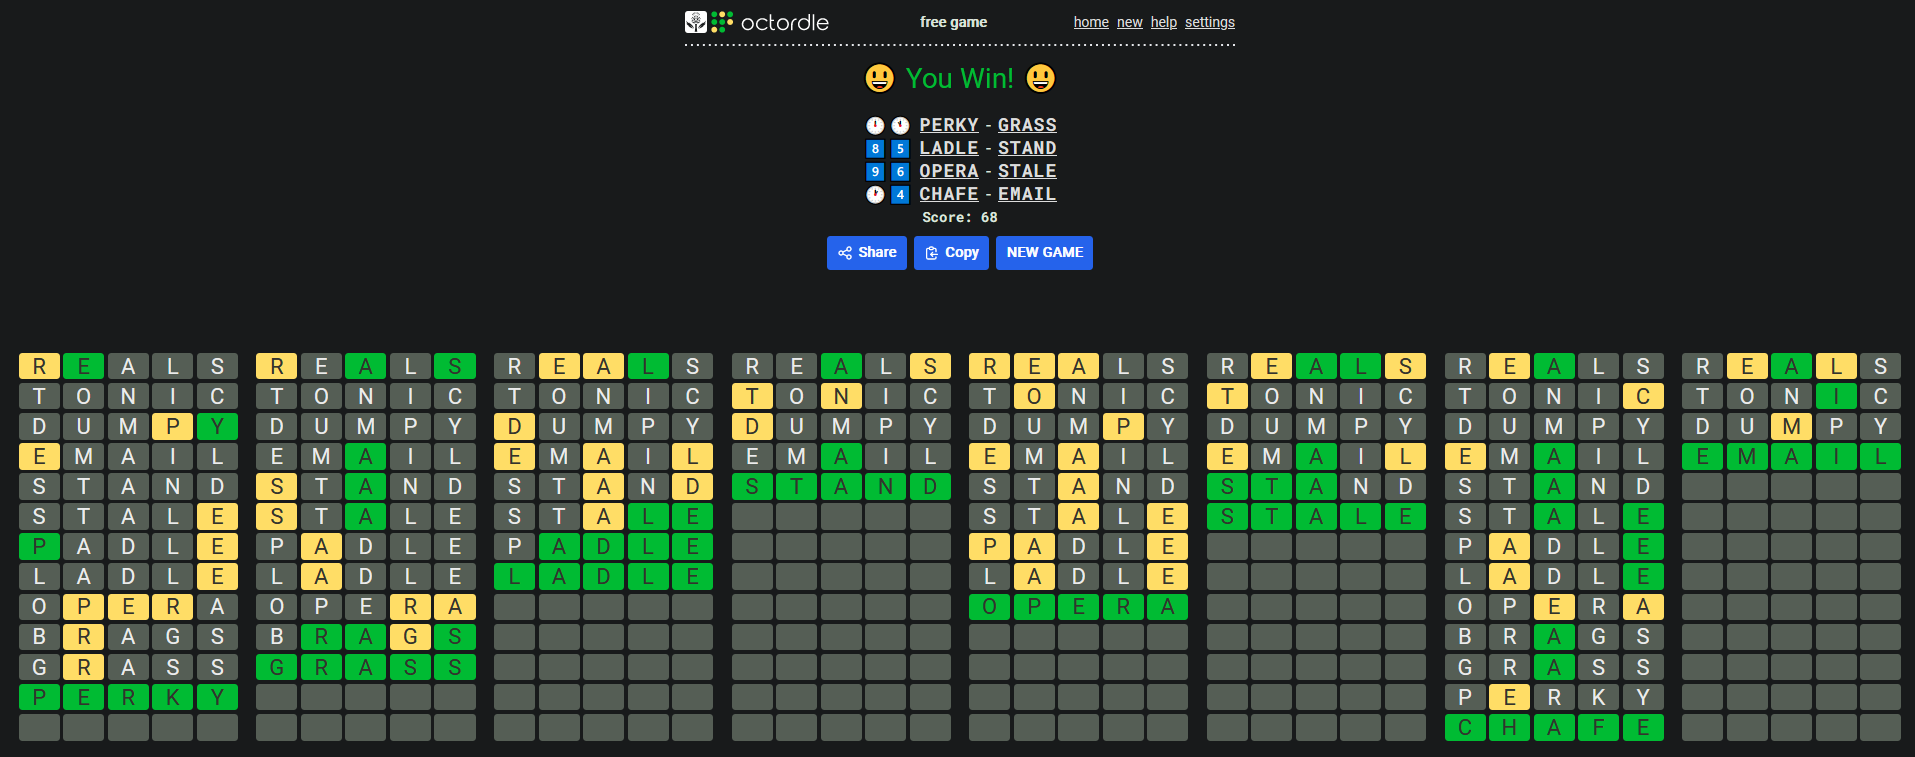
\includegraphics[clip=true,width=\textwidth]{images/octordle.png}


% \afterpage{\blankpage} % puede generar problema en índice de contenidos
% \newpage


% Capítulo 2
\chapter{Objetivos}

\section{Objetivos principales}

Los objetivos principales son:

\begin{itemize}
	\item El aprendizaje de la tecnología de WebSockets en su implementación de cliente y servidor.
	\item La creación de juego \tutor{¿de juego? ¿de un juego? ¿de juegos?} dentro de una página web, manejo de estados \tutor{¿Qué estados? no parece intuitivo al leerlo} y comunicación en tiempo real.
	\item Desarrollar una aplicación web que se pueda usar desde el navegador y desde el móvil, compartiendo el mismo código.
	\item Desplegar la aplicación utilizando herramientas como Docker y Docker Compose.
\end{itemize}


\section{Objetivos secundarios}

Los objetivos secundarios son:

\begin{itemize}
	\item Realizar un sistema de comunicación entre front-end y back-end fuertemente tipado, utilizando Typescript.
	\item Utilizar un desarrollo por sustracción, eliminando partes del juego que no añaden valor, y haciendo que las partes que permanecen se sientan fluidas usando animaciones.
\end{itemize}


\blankpage

% Capítulo 3
\chapter{Contenidos principales}
\label{chap:contenidos}

\section{Primera sección}

% Citar una referencia
Esto es una referencia bibliográfica \cite{bibex}. Se recomienda leer ``The Not So Short Introduction to \LaTeX'' \cite{Oetiker2007} (existen versiones más modernas).


\subsection{Ecuaciones y fórmulas}

Gracias a la ecuación de Euler ($e^{ \pm i\theta } = \cos \theta \pm i\sin \theta$) podemos ver la relación entre varias de las constantes matemáticas más importantes:
\[
    e^{i\pi} + 1 = 0.
\]


% Fórmula numerada
Si una ecuación se va a referenciar es necesario numerarla:
\begin{eqnarray}
\label{eq:schemeP}
 \Phi (k)=\dfrac{2}{|R(k)|(|R(k)|-1)} \underset{i,j \in R(k)}{\sum} a_{ij}.
\end{eqnarray}
Posteriormente se hace referencia a la ecuación a través de su etiqueta (label). Por ejemplo, la anterior ecuación \eqref{eq:schemeP}.



Problema de optimización:
\begin{equation}\label{eq:LP1}
\begin{array}{cl}
  \displaystyle \begin{array}{c}\mathrm{minimizar} \\ \mathbf{t} \in \mathbb{R}^{n}, \  \mathbf{p} \in \mathbb{R}^{m} \end{array} & \hspace{-0.2cm} \begin{array}{c} \mathbf{1}^{\transpuesta}\mathbf{t} \\ \mbox{} \end{array}  \\
  & \vspace{-0.4cm} \\ % línea (fila) en blanco, pero la hacemos estrecha con el comando vspace
  \mbox{sujeto a} & -\mathbf{t} \preceq  \mathbf{V}\mathbf{p} - \mathbf{x}  \preceq  \mathbf{t},\\
 \end{array}
\end{equation}




\subsection{Tablas y figuras}

% Insertar una tabla
\begin{table}
  \centering
  \caption{Título de la tabla.}
  \label{tab:una_tabla}

\begin{footnotesize}
\renewcommand{\arraystretch}{1.5} % Para cambiar la separación entre filas (1 por defecto)
\begin{tabular}{ccccccccccc}
  \hline
   & Subs. & Students & A & PE & WA & RE & CTE & IF & TLE & All\\
  \hline
Ex. 1 & 104 & 44 & 1.27    &   0       &   0.55    &   0.23    &   0.20    &   0.11    &   0     & 2.36  \\
Ex. 2 & 118 & 37 & 0.92    &   0       &   0.92    &   0.27    &   0.49    &   0.59    &   0     & 3.19  \\
Ex. 3 & 100 & 28 & 1.21    &   0.39    &   1.18    &   0.54    &   0.14    &   0.07    &   0.04  & 3.57  \\
Ex. 4 & 78  & 25 & 1.08    &   0.84    &   0.52    &   0.40    &   0.24    &   0.04    &   0     & 3.12  \\
Ex. 5 & 116 & 31 & 1.48    &   0.10    &   0.77    &   0.32    &   0.42    &   0.19    &   0.45  & 3.74  \\
Ex. 6 & 213 & 32 & 1.06    &   0.34    &   3.81    &   0.56    &   0.69    &   0.06    &   0.13  & 6.66  \\
Ex. 7 & 116 & 34 & 1.35    &   0.38    &   0.38    &   0.68    &   0.62    &   0       &   0     & 3.41  \\
  \hline
Average & 120.7 & 33 & 1.20 &  0.26 &  1.14 &  0.42 &  0.40 &  0.16 &  0.08 & 3.66 \\
  \hline
 \end{tabular}
\end{footnotesize}

\end{table}









\begin{sidewaystable}
  \centering
  \caption{Tabla rotada. Factor groupings for the Mooshak questionnaire.}\label{tab:factor_analysis}

\renewcommand{\arraystretch}{1.1}
\begin{scriptsize}
 \begin{tabular}{clcc}
   \hline
   Factor & \textbf{Interpretation} / Items$^{*}$ (loadings)  & Median & Mode \\
   \hline
   \hline
    1 & \multicolumn{3}{l}{\textbf{Students' perception of Mooshak towards its helpfulness in learning} } \\
   \hline
    (21.17\%) & m10. Mooshak has forced me to implement programs more carefully $(0.849)$ & 4 & 4 \\
    $\alpha$ = 0.922 & m6.  Mooshak has helped me improve as a programmer $(0.819)$ & 3 & 4 \\
     & m5.  Mooshak has made me more aware of the need to write correct code $(0.781)$ & 3 & 3\\
     & m1. Mooshak has forced me to program more responsibly $(0.713)$ & 3 & 3 \\
     & m15. The specifications regarding the exercises used with Mooshak are adequate $(0.687)$ & 3 & 3 \\
     & m18. Mooshak helps to measure my current programming skills $(0.680)$ & 2.5 & 3 \\
   \hline
%   \multicolumn{4}{c}{} \vspace{-0.2cm}\\
%   \hline
    2 & \multicolumn{3}{l}{\textbf{Disposition towards using Mooshak} } \\
   \hline
    (17.93\%) & m24. I would be willing to participate in a programming contest using Mooshak, with similar exercises to the ones & 2 & 1 \\
    $\alpha$ = 0.897 & seen throughout the course $(0.807)$ & & \\
    & m13. Using Moohak in the final exams is a good idea $(0.748)$ & 2 & 1 \\
    & m14. I would like to use Mooshak or a similar tool in the future $(0.734)$ & 3 & 1 \\
    & m17. Knowing Mooshak can motivate me to take part in a programming contest $(0.655)$ & 2 & 1\\
    & m9. It would have been useful to use Mooshak from the first programming course $(0.527)$ & 2.5 & 1\\
     & m16. Using Mooshak in the course has been interesting $(0.522)$ & 3 & 4 \\
   \hline
%   \multicolumn{4}{c}{} \vspace{-0.2cm}\\
%   \hline
    3 & \multicolumn{3}{l}{\textbf{Effect of Mooshak's feedback in the tool's usefulness} } \\
   \hline
    (14.84\%) & m12. Mooshak's feedback is adequate $(0.832)$ & 2 & 1\\
    $\alpha$ = 0.836 & m3. Using Mooshak has increased my workload considerably $(0.693)$ & 4 & 4 \\
     & m7.  If Mooshak does not accept my code I feel motivated to find and fix the errors $(0.691)$ & 2 & 3 \\
     & m8.  In general, using Mooshak has been a good idea $(0.666)$ & 3 & 4 \\
   \hline
%   \multicolumn{4}{c}{} \vspace{-0.2cm}\\
%   \hline
    4 & \multicolumn{3}{l}{\textbf{Mooshak's effect on persistence} } \\
   \hline
    (11.20\%) & m23. When Mooshak does not accept my code I get discouraged and I abandon the exercise $(0.848)$ & 3 & 3 \\
    $\alpha$ = 0.705 & m22. Mooshak has been a waste of time $(0.597)$ & 2 & 2 \\
    & m25. Once a program has passed Mooshak's tests, I rewrite it in order to enhance it $(0.559)$ & 2 & 2 \\
   \hline
%   \multicolumn{4}{c}{} \vspace{-0.2cm}\\
%   \hline
   5 & \multicolumn{3}{l}{\textbf{Students' perception of Mooshak's features} } \\
   \hline
    (10.87\%) & m20. Even if it is not related to the grade, I feel satisfied if I am one of the first students to complete an exercise $(0.729)$ & 2 & 2\\
   $\alpha$ = 0.742  & m19. I value the fact that a tool like Mooshak returns feedback in real time about the correction of my programs $(0.650)$ & 3.5 & 4 \\
   \hline
%   \multicolumn{4}{c}{} \vspace{-0.2cm}\\
%   \hline
\multicolumn{4}{l}{\scriptsize $^{*}$Measured on a 5-point Likert scale (1: strongly disagree; 2: disagree; 3: neutral; 4: agree; 5: strongly agree).}
  \end{tabular}
\end{scriptsize}
\end{sidewaystable}



\begin{table}
  \centering

\begin{small}
\begin{tabular}{|l|l|l|l|}\hline
  \multirow{10}{*}{numeric literals} & \multirow{5}{*}{integers} & in decimal & \verb|8743| \\ \cline{3-4}
  & & \multirow{2}{*}{in octal} & \verb|0o7464| \\ \cline{4-4}
  & & & \verb|0O103| \\ \cline{3-4}
  & & \multirow{2}{*}{in hexadecimal} & \verb|0x5A0FF| \\ \cline{4-4}
  & & & \verb|0xE0F2| \\ \cline{2-4}
  & \multirow{5}{*}{fractionals} & \multirow{5}{*}{in decimal} & \verb|140.58| \\ \cline{4-4}
  & & & \verb|8.04e7| \\ \cline{4-4}
  & & & \verb|0.347E+12| \\ \cline{4-4}
  & & & \verb|5.47E-12| \\ \cline{4-4}
  & & & \verb|47e22| \\ \cline{1-4}
  \multicolumn{3}{|l|}{\multirow{3}{*}{char literals}} & \verb|'H'| \\ \cline{4-4}
  \multicolumn{3}{|l|}{} & \verb|'\n'| \\ \cline{4-4}          %% here
  \multicolumn{3}{|l|}{} & \verb|'\x65'| \\ \cline{1-4}        %% here
  \multicolumn{3}{|l|}{\multirow{2}{*}{string literals}} & \verb|"bom dia"| \\ \cline{4-4}
  \multicolumn{3}{|l|}{} & \verb|"ouro preto\nmg"| \\ \cline{1-4}          %% here
\end{tabular}
\end{small}

  \caption{Tabla con ``multicolumnas'' y ``multifilas''.}\label{tab:tablacompleja}
\end{table}





% Insertar una figura
\begin{figure}
  \centering
  \includegraphics[width=0.75\textwidth,clip=true]{\logoUniversidad}
  \caption{Logo de la Universidad.}
  \label{fig:logo_universidad}
\end{figure}

% Referenciar una etiqueta (label)
Las tablas y figuras deben presentarse en el texto, referenciadas y numeradas. La descripción de una figura debe ir posicionada debajo de la misma. Las descripciones de tablas pueden aparecer encima o debajo de las mismas (pero de forma consistente en todo el documento).

En las tablas se recomienda evitar líneas verticales y usar pocas horizontales. 

La figura~\ref{fig:logo_universidad} se utiliza en la portada. \LaTeX ubica automáticamente las tablas y figuras. Para ello emplea reglas basadas en la experiencia de profesionales de la edición de textos. Podemos forzar su ubicación, pero en general es recomendable usar la ubicación sugerida por el sistema \LaTeX. Usad gráficos vectoriales siempre que podáis.





\begin{figure}
   \centering

  \begin{minipage}{0.45\textwidth}
   \centering

     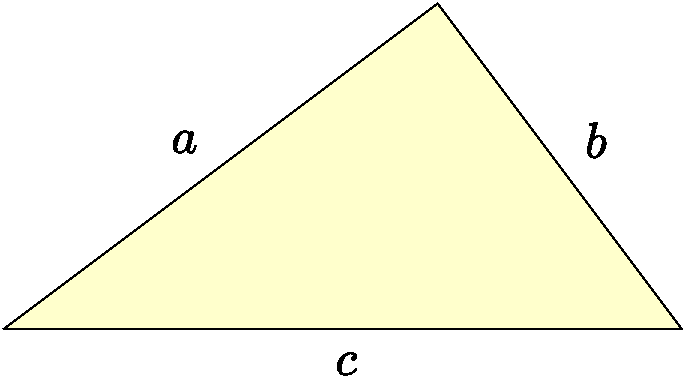
\includegraphics[clip=true,width=\textwidth]{triangulo_grande_bb.pdf}\\

    \footnotesize (a)
  \end{minipage}
  \hfill
  \begin{minipage}{0.45\textwidth}
   \centering
     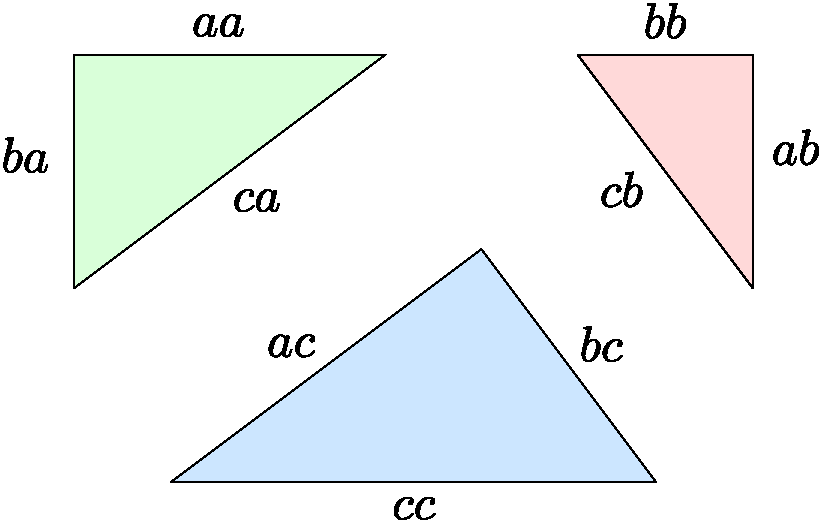
\includegraphics[clip=true,width=\textwidth]{triangulos_separados_bb.pdf}\\

   \footnotesize (b)
  \end{minipage}

    \bigskip

    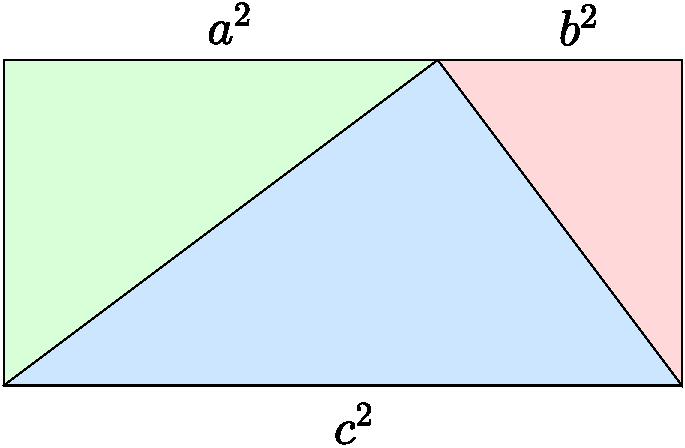
\includegraphics[clip=true,width=0.5\textwidth]{triangulos_unidos_bb.pdf}\\
    \footnotesize (c)

  \caption{Ejemplo con varias figuras. Demostración visual del teorema de Pitágoras. En (a) tenemos un triángulo rectángulo con hipotenusa $c$ y catetos $a$ y $b$. En (b) se muestra tres copias escaladas del mismo triángulo. El verde se ha escalado por $a$, el rojo/rosa por $b$, y el azul por $c$. En (c) se juntan los triángulos de (b) para formar un rectángulo cuya base es $c^{2}$, pero también $a^{2} + b^{2}$. Por tanto, $a^{2} + b^{2} = c^{2}$.}\label{fig:teoremapitagoras}
\end{figure}





\section{Segunda sección}

% Nueva página
Normalmente no tendremos que insertar saltos de página, salvo para forzar que los capítulos empiecen en páginas impares, con \begin{verbatim}\blankpage\end{verbatim} En cualquier caso, podemos introducir un salto de página con el comando \begin{verbatim}\newpage\end{verbatim}.

\newpage
% También con \pagebreak



\subsection{Código}


\begin{mypython}[float={!t},caption={Titulo del algoritmo/código.},label={alg:etiqueta}]
def sum_list_limits_1(a, lower, upper):
    if lower > upper:
        return 0
    else:
        return a[upper] + sum_list_limits_1(a, lower, upper - 1)
\end{mypython}
El código~\ref{alg:etiqueta} es un ejemplo en Python.



\begin{algorithm}
\begin{algorithmic}[1]
\STATE $\forall i \in V$, \ let $i$ be an isolated community
\STATE $o=permutation(V)$
\FOR{$k \ \in \ o$}
\STATE search in $A$ all the neighbours of $k$, $j$
\STATE $\forall j$, calculate $\Delta Q_k(j)$ in matrix $\mathcal{M}$
\STATE $j^*=\{ \ j \ | \ \Delta Q_k(j^*)=\max_j\{Q_k(j)\} \ \}$
\IF{$\Delta Q_k(j^*)>0$}
\STATE{Move node $k$ to $j^*$ 's community}
\ELSE
\STATE{$k$ remains in its community}
\ENDIF
\ENDFOR
\end{algorithmic}\caption{\textit{Additional Louvain} \textbf{input}=$\left(A, \ \mathcal{M}\right)$ \textbf{output}=$P$}
\label{alg:AdditionalLouvain}
\end{algorithm}
En el algoritmo~\ref{alg:AdditionalLouvain} aparece un ejemplo en pseudocódigo.

% Capítulo 4
\chapter{Descripción informática}
\section{Requisitos}
Como la metodología de desarrollo ha sido iterativa, algunos de los requisitos han ido surgiendo durante el desarrollo de la aplicación, e inclusos algunos requisitos han cambiado según se han ido encontrando o destruyendo barreras. Los requisitos iniciales, que se plantearon en la primera reunión eran:

Desarrollar una aplicación para cuatro jugadores en las que compiten para encontrar la palabra. En este momento ya se ha definido que es un juego variante del Wordle, además, por simplificar el desarrollo en estos momentos iniciales, se ha decidido guardar la información sobre los jugadores en memoría, sin utilizar ninguna base de datos.

\subsection{Fases}
En cada fase de desarrollo quedan agrupadas una serie de nuevos requisitos y mejoras sobre los requisitos que ya se habían completado.

\subsubsection{Fase 0}
En la fase 0, se propone la idea de la aplicación y se comienzan a crear requisitos, primero se define las ideas y los requerimientos, como la necesidad de crear un sistema de tiempo real, además, se especifican las tecnologías, y se define como debería de avanzar el proyecto a lo largo del tiempo.

\subsubsection{Fase 1}
En la fase 1, se presentó una primera versión de la aplicación, en ella un número no controlado de jugadores podían jugar en una misma sala, existía un lobby donde los jugadores podían cambiar su nombre y podían jugar hasta que uno ganase. Todavía no se llegaba a controlar el que los jugadores hubieran perdido, así que era posible quedarse bloqueado con todos los jugadores sin posibilidad de probar nuevas palabras.
La palabra objetivo en esta fase no era generada aleatoriamente, en su lugar, era siempre la misma palabra. Esto facilitaba mucho las pruebas iniciales de flujo de la aplicación.

\subsubsection{Fase 2}
En la fase 2, el servidor ya era capaz de generar una palabra aleatoria entre una lista de posibles palabras. Todos los jugadores reciben la palabra objetivo aleatoria al comenzar la partida, en el momento en el que uno de ellos ganaba, se mostraba su nombre y la palabra objetivo en una nueva página.
	      	      	      	      	      	      	      	      
La página que muestra al jugador ganador, como el resto de páginas, fue cambiando a lo largo del tiempo, sobre ella se hicieron muchas iteraciones que permitieron llegar al diseño final.

\subsubsection{Fase 3}
En la fase 3, se introdujo la opción de unir a traves del boton de Join del menú principal, además, se introdujo la posibilidad de ver en tiempo real el conocimiento adquirido de cada jugador sobre la palabra objetivo y se amplió la lista de palabras para que soportara diferentes idiomas, en concreto se introdujo el idioma español, pero el sistema es capaz de introducir nuevas listas de palabras de manera sencilla.
	      	      	      	      
Además, se prestó especial atención a casos donde hay un único jugador en la partida, por ejemplo, para estos casos se eliminó la cuenta atrás del principio de la partida.
	      	      	      	      	
Para poder probar con amigos y compañeros de trabajo, se desplegó la aplicación moviendo las aplicaciones a un servidor de DigitalOcean, levantando ambas aplicaciones utilizando los comandos que proveen tanto SvelteKit como Deno. Esta forma de levantar las aplicaciones se demostró muy lenta, ya que requería actualizar los repositorios del servidor usando Git, para después compilar y ejecutar las aplicaciones.

\subsubsection{Fase 4} Para la fase 4, se arreglaron bugs presentes, además se desarrolló la posibilidad de levantar la aplicación utilizando Docker y Docker Compose.

En este momento la aplicación ya se encontraba con madurez suficiente para que los cambios necesarios fueran aplicados sin necesidad de hacer refactorizaciones ni grandes cambios en los sistemas de la aplicación.    	      	      	      	      	


\section{Arquitectura general}
El proyecto está dividido en dos repositorios, por un lado está la aplicación web (webapp), que se encarga de realizar la lógica de presentación, así como el game loop, y por otro lado tenemos el servidor de backend, donde va toda la lógica de websockets en la parte de servidor.

La comunicación entre aplicaciones se realiza mediante peticiones HTTP y websockets, para ello se utiliza la librería estándar de Javascript proporcionada por el navegador, la librería estándar de Node.js, la librería estándar de Deno y la librería Socket.io.


\begin{center}
	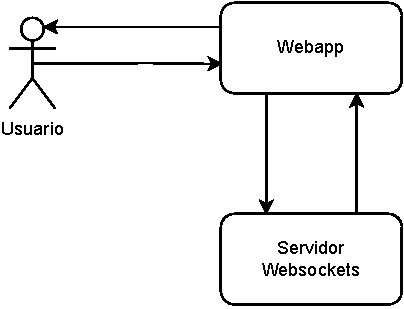
\includegraphics[clip=true,width=0.5\textwidth]{./diagrams/general_arch.pdf}
\end{center}

\subsection{Aplicación web}
La aplicación web es la herramienta con la cual el usuario interactúa, permite a este realizar todas las acciones necesarias utilizando un navegador web.

Está desarrollada utilizando SvelteKit para la realización de la lógica, y Tailwind para dar color y estilo.

El flujo principal que sigue el usuario para poder jugar una partida comienza abriendo la página web de la aplicación web, después, creará o se unirá a una partida ya creada, cuando todos los jugadores estén listos, el creador de la partida le dará al botón de comenzar, y después de una cuenta atrás, a todos los jugadores se les presentará un tablero de Wordle donde pondrán ir escribiendo sus intentos. Si alguno de los jugadores descubre la palabra, todos los jugadores verán una nueva pantalla con el nombre de la persona ganadora, en esta nueva pantalla, los jugadores pueden elegir entre salir de la partida o volver a jugar. En caso de que ningún jugador consiga ganar, se les presentará a todos una pantalla en el que se mostrará la palabra objetivo, y las mismas opciones que en el caso de haber habido un ganador.


\begin{center}
	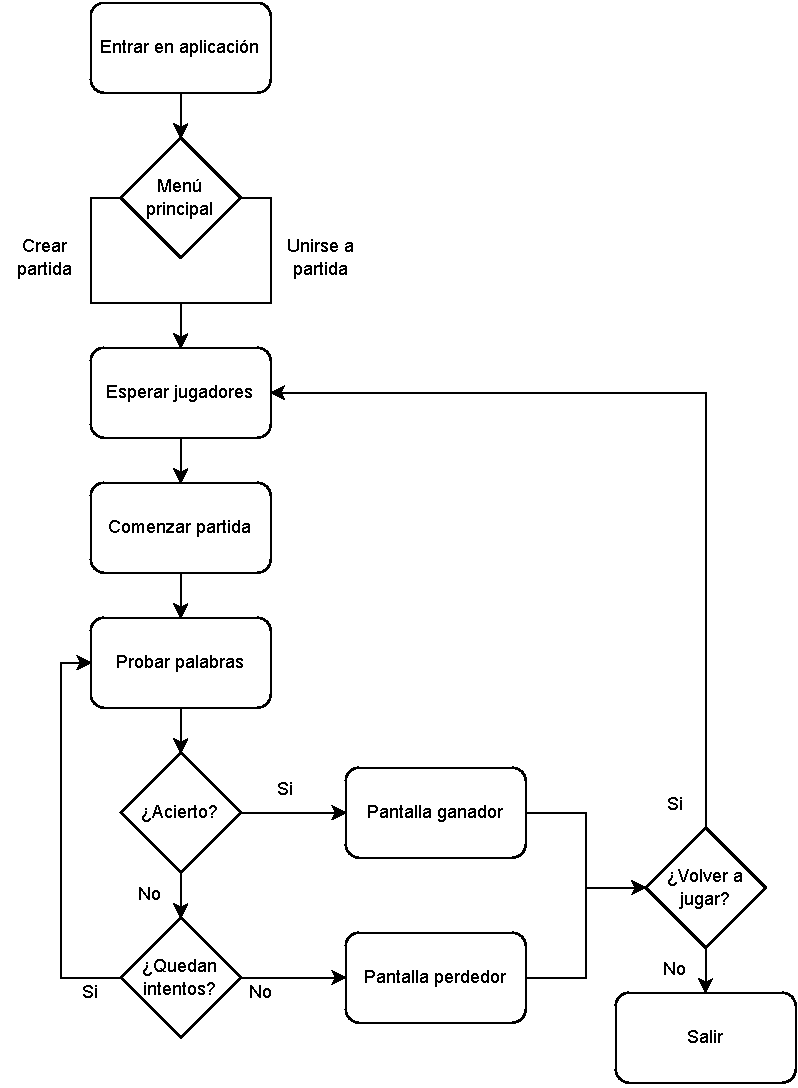
\includegraphics[clip=true,width=\textwidth]{./diagrams/webapp_flow.pdf}
\end{center}

\subsubsection{Comunicación websocket}
La comunicación websocket ha sido el punto de aprendizaje principal, según se fueron desarrollando las diferentes partes para el trabajo, se fue definiendo lo que acabó siendo una serie de reglas sobre la comunicación diferenciando estas en tres tipos de comunicación diferentes.

Para entender estos tres tipos de comunicación hay que entender primero el sistema de comunicación HTTP. En este tipo de comunicación es el cliente el que inicia la llamada y es el servidor el que responde a esta. Sin embargo, en websockets, el servidor puede enviar información al cliente sin que sea el iniciador de la llamada. Por ello Websockets funciona por sistemas de eventos, donde el socket puede enviar y esperar comunicación (comunicación bidireccional).

Una vez entendida la comunicación HTTP y la comunicación websocket, y las diferencias entre ambas, va a quedar claro porque en CoWordle se diferencia entre tres tipos distintos de comunicación.

En primer lugar tenemos la comunicación cliente - servidor, donde el cliente envía eventos al servidor, y el servidor puede actuar ante estos eventos, pero no responde a través de ellos. 
Estos eventos se clasifican como eventos OUT, ya que el cliente envía información al exterior. Por ejemplo, la llamada cuando un jugador ha sido expulsado de la partida (\textit{remove\_player}), se envía desde el host de la partida hacia el servidor, cuando el servidor ha procesado este evento, envía a todos los jugadores de la partida el evento \textit{player\_disconnected}, y serán los clientes los que eliminen de sus listados locales al jugador que se ha eliminado.

En segundo lugar tenemos la comunicación servidor - cliente, un ejemplo de esto es el recién descrito \textit{player\_disconnected}, en el que el servidor envía un evento a los jugadores de la sala. Este tipo de eventos se clasifica en CoWordle como IN, porque el cliente recibe información del servidor.

Por último lugar el último tipo de comunicación se clasifica como DIALOGUE, y se explica porque es comunicación cliente - servidor - cliente, es decir, es el cliente el que comienza la comunicación, el servidor procesa la respuesta y se la envía al cliente con el mismo nombre de evento con el que la llamada había comenzado, hasta que la llamada no ha sido respondida, el cliente se quedará esperando una respuesta de manera asíncrona, es decir, sin bloquear al resto de la aplicación.

\subsection{Servidor Websockets}
El servidor de websockets está implementado utilizando Deno y una librería que ayuda al manejo de eventos para los websockets llamada Socket.io. Deno se utiliza para levantar el servidor y para recibir peticiones HTTP, aunque existen pocos endpoints para la comunicación HTTP, existe un endpoint necesario para que Socket.io cree la conexión de Websockets, y uno más para la creación de la partida.

\subsubsection{Sistema de eventos}
El servidor responde a peticiones HTTP y de Websockets creando eventos que son respondidos de manera secuencial por funciones lambda, cada función sólo responde a un evento, devolviendo una respuesta.
Javascript es una tecnología uni-hilo, pero es capaz de realizar concurrencia utilizando primitivas asíncronas llamadas promesas, cuando una función marcada como asíncrona se ejecuta, el motor de Javascript la guarda como evento, este evento será manejado cuando el motor de Javascript lo considere oportuno. Por ejemplo, cuando la CPU está esperando una lectura de la memoría, Javascript puede cambiar el contexto y procesar otras funciones. De está manera, Javascript es capaz de maximizar la utilización de su hilo de ejecución.

\subsubsection{Eventos disponibles}
El servidor permite la comunicación utilizando las siguientes rutas HTTP:Soso

\begin{itemize}
	\item \textit{/create-route}, genera un nuevo identificador de partida. Este identificador es fundamental para la comunicación entre el cliente y el servidor ya que permite la identificación de la partida para realizar las operaciones necesarias.
	\item \textit{/testing/solution}, este endpoint está disponible para poder realizar un tests de integración de flujo completo.correcta.
\end{itemize}

A parte de las rutas HTTP, el servidor permite la comunicación Websocket utilizando los siguientes eventos:

\begin{itemize}
	\item \textit{setup} es un evento de tipo diálogo que une a un jugador a la partida, es necesario enviar como parámetros el código de la sala generado por /create-room y el nombre del usuario que se va a unir a la partida, este evento avisa a todos los demás jugadores de la sala que se ha unido el jugador emitiendo el evento \textit{player\_connection}.
	\item \textit{update\_player\_name} es un evento de tipo diálogo que permite a los jugadores actualizar su nombre, especialmente útil porque el primer nombre que recibe cada jugador al conectarse a la partida es aleatorio entre una combinación de posibilidades.
	\item \textit{remove\_player} es un evento de tipo out que solo pueden utilizar el creador de la partida, y permite expulsar a jugadores de la partida. Cuando ha expulsado a un jugador emite un evento \textit{player\_disconnected} que notifica al resto de usuarios de la desconexión.
	\item \textit{validate\_word} es un evento de tipo diálogo que comprueba un intento de un jugador con la palabra objetivo. El resultado de la operación de comprobación es un array de una enumeración (\textit{WordlePoints}) que indican el resultado de cada letra en la palabra (si no se encuentra en la palabra, si se encuentra en la palabra, si está en la posición correcta). Este resultado se envía directamente al jugador que ha ejecutado el evento, pero también se envía a los demás jugadores para indicar en el scoreboard el conocimiento de cada jugador. Además, se comprueba si la partida ha terminado por que el intento coincide con la palabra objetivo, y si todos los jugadores han perdido porque se han quedado sin intentos.
	\item \textit{start\_game} es un evento de tipo out que permite al host de la partida empezar. En el momento que se lanza este evento todos los jugadores reciben el evento \textit{start\_prematch} que les indica cuándo comenzará la partida.
	\item \textit{disconnect} es un evento nativo de Socket.io, que permite al servidor conocer cuando un jugador se ha desconectado de la partida, existen varias razones para que se ejecute este evento, por ejemplo, que el jugador haya perdido la conexión con internet, o que el jugador haya decidido abandonar la partida cerrando el navegador. En este evento se comunica al resto de jugadores que este ha abandonado la partida, en caso de ser el jugador que ha creado la partida el que la abandona, se cierra también para el resto de jugadores.
\end{itemize}


\subsubsection{Endpoints HTTP}
Como el objetivo del trabajo era el aprendizaje de la comunicación bidireccional, la mayor parte de la comunicación se realiza a traves de websockets, aun asi existen dos rutas disponibles para la realización de comunicación HTTP:

\begin{itemize}
	\item \textit{/create-room} crea una nueva partida para que los jugadores puedan unirse y jugar. Cada partida está identificada por un identificador que se genera durante este proceso.
	\item Existe también una ruta reservada por la librería de Socket.IO que se utiliza internamente para establecer la conexión websocket. Esta ruta está completamente manejada por Socket.IO.
\end{itemize}

\subsubsection{Identificador de partida}
Cada partida tiene un identificador único de seis cifras generado pseudo-aleatoriamente llamado roomCode. El roomCode lo generará el servidor de websockets tras la petición de /create-room, este endpoint HTTP únicamente reserva el código generado para la partida, utilizando ese código los jugadores son capaces de unirse a la partida inicialmente, el código también se utiliza para realizar la comunicación cliente-servidor.


\section{Diseño e Implementación}

\subsection{La reutilización de componentes}
Svelte, la tecnología que he usado para hacer los componentes de front, se basa en la creación de componentes que puedan ser reutilizados en diferentes situaciones, la reutilización de código se considera buena práctica en todo el ámbito de la ingeniería informática. Por ello parece importante destacar que una buena elección de la tecnologías es solo la base, y es necesario hacer un buen uso de estas para poder llegar a un buen resultado, por ello en este apartado quiero destacar un buen uso de componentes de Svelte.

Existe un componente que se reutiliza varias veces a lo largo de la aplicación, el componente llamado <Word>, que se encuentra en el archivo Word.svelte de la aplicación cowordle-webapp.

Este componente se utiliza como botones estilizados en el menú principal, en este primer uso, el componente muestra la palabra elegida por el desarrollador, indicando al usuario que es un botón con el que puede interaccionar.

\begin{figure}[H]
	\centering
	
\includegraphics[clip=true]{images/reusing/host_component.png}
	\caption{Imagen del componente como botón.}
	\label{fig:comp_host_image}
\end{figure}

Después, se vuelve utilizar como huecos para las palabras mientras se juega, en este caso la palabra tiene distinto número de huecos disponibles, además está completamente vacía de texto.

\begin{figure}[H]
	\centering
	
\includegraphics[clip=true, width=0.75\textwidth]{images/reusing/empty_component.png}
	\caption{Imagen del componente con texto vacio.}
	\label{fig:comp_empty}
\end{figure}


Cuando el jugador interacciona con el teclado mientras juega, las palabras se van llenando de letras.

\begin{figure}[H]
	\centering
	
\includegraphics[clip=true, width=0.75\textwidth]{images/reusing/filled_component.png}
	\caption{Imagen del componente con texto.}
	\label{fig:comp_filled}
\end{figure}

Además, las letras muestran el progreso de la palabra objetivo, utilizando los colores característicos.

\begin{figure}[H]
	\centering
	
\includegraphics[clip=true, width=0.75\textwidth]{images/reusing/colored_component.png}
	\caption{Imagen del componente con texto y colores.}
	\label{fig:comp_colored}
\end{figure}

Todas las imágenes mostradas representan el mismo componente de Svelte, y permiten mostrar las ventajas de utilizar tecnologías web reactivas.
Comenzando por el principio, necesitamos un componente que sea capaz de mostrar texto.

\begin{figure}[H]
	\centering
	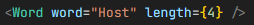
\includegraphics[clip=true, width=0.75\textwidth]{images/reusing/code_simple_component.png}
	\caption{Imagen código para utilizar el componente.}
	\label{fig:comp_simple_code}
\end{figure}

Así es como se utiliza el componente Word, para mostrar el texto de la primera imagen simplemente es necesario definir la palabra a mostrar y su longitud.

También queremos que el componente reciba texto del usuario dinámicamente, esto sería posible reprogramando al componente o creando uno nuevo, pero realmente ya tenemos esta funcionalidad sin necesidad de programar nada más. En lugar de utilizar como argumento para el parámetro word un string fijo, podemos utilizar una variable, e indicarle a Svelte que esa variable es reactiva utilizando, la directiva bind, que recalcula el componente cada vez que cambia el contenido de la variable pasada.

\begin{figure}[H]
	\centering
	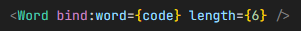
\includegraphics[clip=true, width=0.75\textwidth]{images/reusing/code_dyn_component.png}
	\caption{Imagen código para utilizar el componente con texto dinámico.}
	\label{fig:comp_dyn_code}
\end{figure}

En este caso estamos utilizando la directiva bind para hacer que el componente se redibuje cada vez que cambia la variable code. Esto significa que nuestro componente es ajeno al texto que presentamos, y es responsabilidad de otros componentes seleccionar el texto a mostrar.

Parece un pequeño detalle, pero esta flexibilidad de desarrollo simplifica el código haciéndolo muy reutilizable y componible.

La primera implementación del componente Word se hizo cuando se comenzó el proyecto,  y sin mucho cambio, ha llegado a utilizarse en otras partes de la aplicación en las que no se había llegado a pensar cuando se creó el componente, y eso demuestra que se realizó un buen diseño inicialmente.


\blankpage


% Nuevo capítulo
% \chapter{Resultados (opcional)}
% \label{sec:resulObtenidos}

% En esta sección se describe los resultados obtenidos en el TFG, en caso de realizar propuestas para su resolución. Puede sustituirse por ejemplos u omitirse.


% \blankpage

% Nuevo capítulo

\chapter{Conclusiones y trabajos futuros}

En este capítulo se detallan las conclusiones derivadas del TFG y la propuesta de posibles trabajos futuros.

Las citas del texto Autor \cite{giaquinta}, Autor \cite{fortune}, Autor \cite{fortuneB}, Autor \cite{mitchell} y Autor \cite{morrey} deben ir referenciadas en la bibliografia.


\section{Texto de relleno}

\lipsum[1-18]

\blankpage


%%%%%%%%%%%%%%%%%%%%%%%%%%%%%%% Bibliografía %%%%%%%%%%%%%%%%%%%%%%%%%%%%%%%

\phantomsection
\addcontentsline{toc}{chapter}{Bibliografía}

\footnotesize{
	%\bibliographystyle{hispa}
	\bibliographystyle{IEEEtran}
	\bibliography{bibliografia}
}



% No expandir elementos para llenar toda la página
\raggedbottom
\afterpage{\blankpage}

\newpage




%%%%%%%%%%%%%%%%%%%%%%%%%%%%%%% Apéndices %%%%%%%%%%%%%%%%%%%%%%%%%%%%%%%

% \appendix

% \phantomsection
% \addcontentsline{toc}{chapter}{Apéndices}

% \mbox{}
% \vfill
% \begin{center}
% 	\begin{Huge}
% 		\textbf{Apéndices}
% 	\end{Huge}
% \end{center}
% \vfill
% \mbox{}
% \thispagestyle{empty}

% \newpage
% \mbox{}
% \thispagestyle{empty}
% \newpage


% Primer apéndice
% \chapter{Este es el primer apéndice}
% \label{sec:apendice}

% \section{Ejemplo de sección}

Sección del apéndice


% Fin del documento
\end{document}
